\documentclass[11pt,a4paper]{article}

\usepackage[margin=0.82in]{geometry}
\usepackage[T1]{fontenc}
\usepackage{lmodern}
\usepackage{microtype}
\usepackage{amsmath,amssymb}
\usepackage{graphicx}
\usepackage{booktabs}
\usepackage{tabularx}
\usepackage{float}
\usepackage{xcolor}
\usepackage[hidelinks]{hyperref}

\setlength{\parskip}{0.45em}
\setlength{\parindent}{0pt}
\renewcommand{\arraystretch}{1.18}
\definecolor{deepteal}{HTML}{176B87}

\title{Assignment 4: Auction Mechanisms\\\large Simulation and Incentive Analysis}
\author{}
\date{November 5, 2026}

\begin{document}
\maketitle

\begin{abstract}
This report studies second-price auctions with one and two rivals, first-price bidding against equilibrium rivals, and VCG procurement of a least-cost path. Monte Carlo estimates are compared with analytical predictions. The second-price experiments support truthful bidding as a best response across the tested rival strategies. In the first-price experiment, the highest tested expected utility occurs near the equilibrium bid multiplier. The VCG example selects path ABEF, pays the three selected edges 4, 2, and 3, and gives no profitable gain from either tested cost misreport.
\end{abstract}

\section{Experimental setup}

The simulations follow the supplied assignment brief \cite{assignment4}. Random private values are independently drawn from the uniform distribution on $[0,1]$. The scripts use NumPy's seeded random-number generator. For each second-price value/strategy combination, 100,000 rival bid samples are reused across the 101 focal bids; this common-random-number design makes neighboring payoff estimates less noisy while preserving the Monte Carlo expectation. Part 2 uses 200,000 auctions for each number of bidders.

The brief's Part 1C sentence says to repeat ``parts A and C.'' I interpret this as ``parts A and B,'' so the two-rival implementation includes both the stochastic payoff sweeps and the fixed-rival truthfulness check. For that check, both rivals use the listed fixed bid. Tied highest bids split the allocation uniformly.

Part 2 does not specify bidder 1's value, although it specifies that the other bidders draw uniform values. I hold bidder 1's value at $v=0.5$, matching the experiment command, and state the result so this assumption is visible. The tested multipliers are $k=0.1,0.2,\ldots,2.0$. The ``could have paid less and still won'' statistic counts auctions in which the winner's bid exceeds the runner-up bid by more than a numerical tolerance. I also report the average bid gap, since the fraction is nearly always one under continuous random bids.

For Part 3, I use the directed edge costs in the transportation network referenced by the handout and the VCG pivot payment rule. When route costs tie during a misreport sweep, the lexicographically earlier node path is selected to make the result deterministic.

\section{Second-price auction}

Bidder 1 wins when its bid $b$ is at least the highest rival bid $Y$ and then pays $Y$. Its utility in a given auction is $v-Y$ if it wins and zero otherwise. The expected utility is therefore
\[
  U(b)=\mathbb{E}\left[(v-Y)\,\mathbf{1}\{Y\leq b\}\right].
\]

\subsection{One rival: stochastic strategies}

With one rival, truthful bidding and random bidding independent of value both produce a uniform rival bid on $[0,1]$. Their theoretical curves are identical:
\[
  U_{\text{uniform}}(b)=vb-\frac{b^2}{2}.
\]
When the rival bids half its value, its bid is uniform on $[0,0.5]$, giving
\[
  U_{\text{half}}(b)=
  \begin{cases}
    2vb-b^2, & 0\leq b\leq 0.5,\\
    v-0.25, & 0.5\leq b\leq 1.
  \end{cases}
\]
The uniform-bid curve is maximized at $b=v$. Against half-value bids, $b=v$ is optimal for $v\leq 0.5$; for $v>0.5$, all bids at least $0.5$ give the same maximum because the rival never bids above $0.5$.

Figure~\ref{fig:part1a} shows the nine simulated curves. The observed maxima occur at the truthful bid for truthful and random rivals. For half-value rivals, the maximizing bid is $0.20$ when $v=0.20$, and any grid bid from $0.50$ through $1.00$ when $v=0.50$ or $0.80$. Thus truthful bidding is a best response for all tested rival models, though in some half-value cases it is not the unique best response. The random-bid and truthful-rival estimates differ slightly because they use independent samples, but both track the same theoretical curve.

\begin{table}[H]
\centering
\caption{Maximum estimated utility in Part 1A (100,000 auctions per case).}
\label{tab:part1a}
\small
\begin{tabular}{ccccc}
\toprule
Value $v$ & Truthful rival & Half-value rival & Random-bid rival & Maximizing bids\\
\midrule
0.20 & 0.019873 & 0.039799 & 0.020154 & $0.20$\\
0.50 & 0.124927 & 0.250227 & 0.125363 & $0.50$; half: $[0.50,1.00]$\\
0.80 & 0.320888 & 0.549808 & 0.321576 & $0.80$; half: $[0.50,1.00]$\\
\bottomrule
\end{tabular}
\end{table}

\begin{figure}[H]
  \centering
  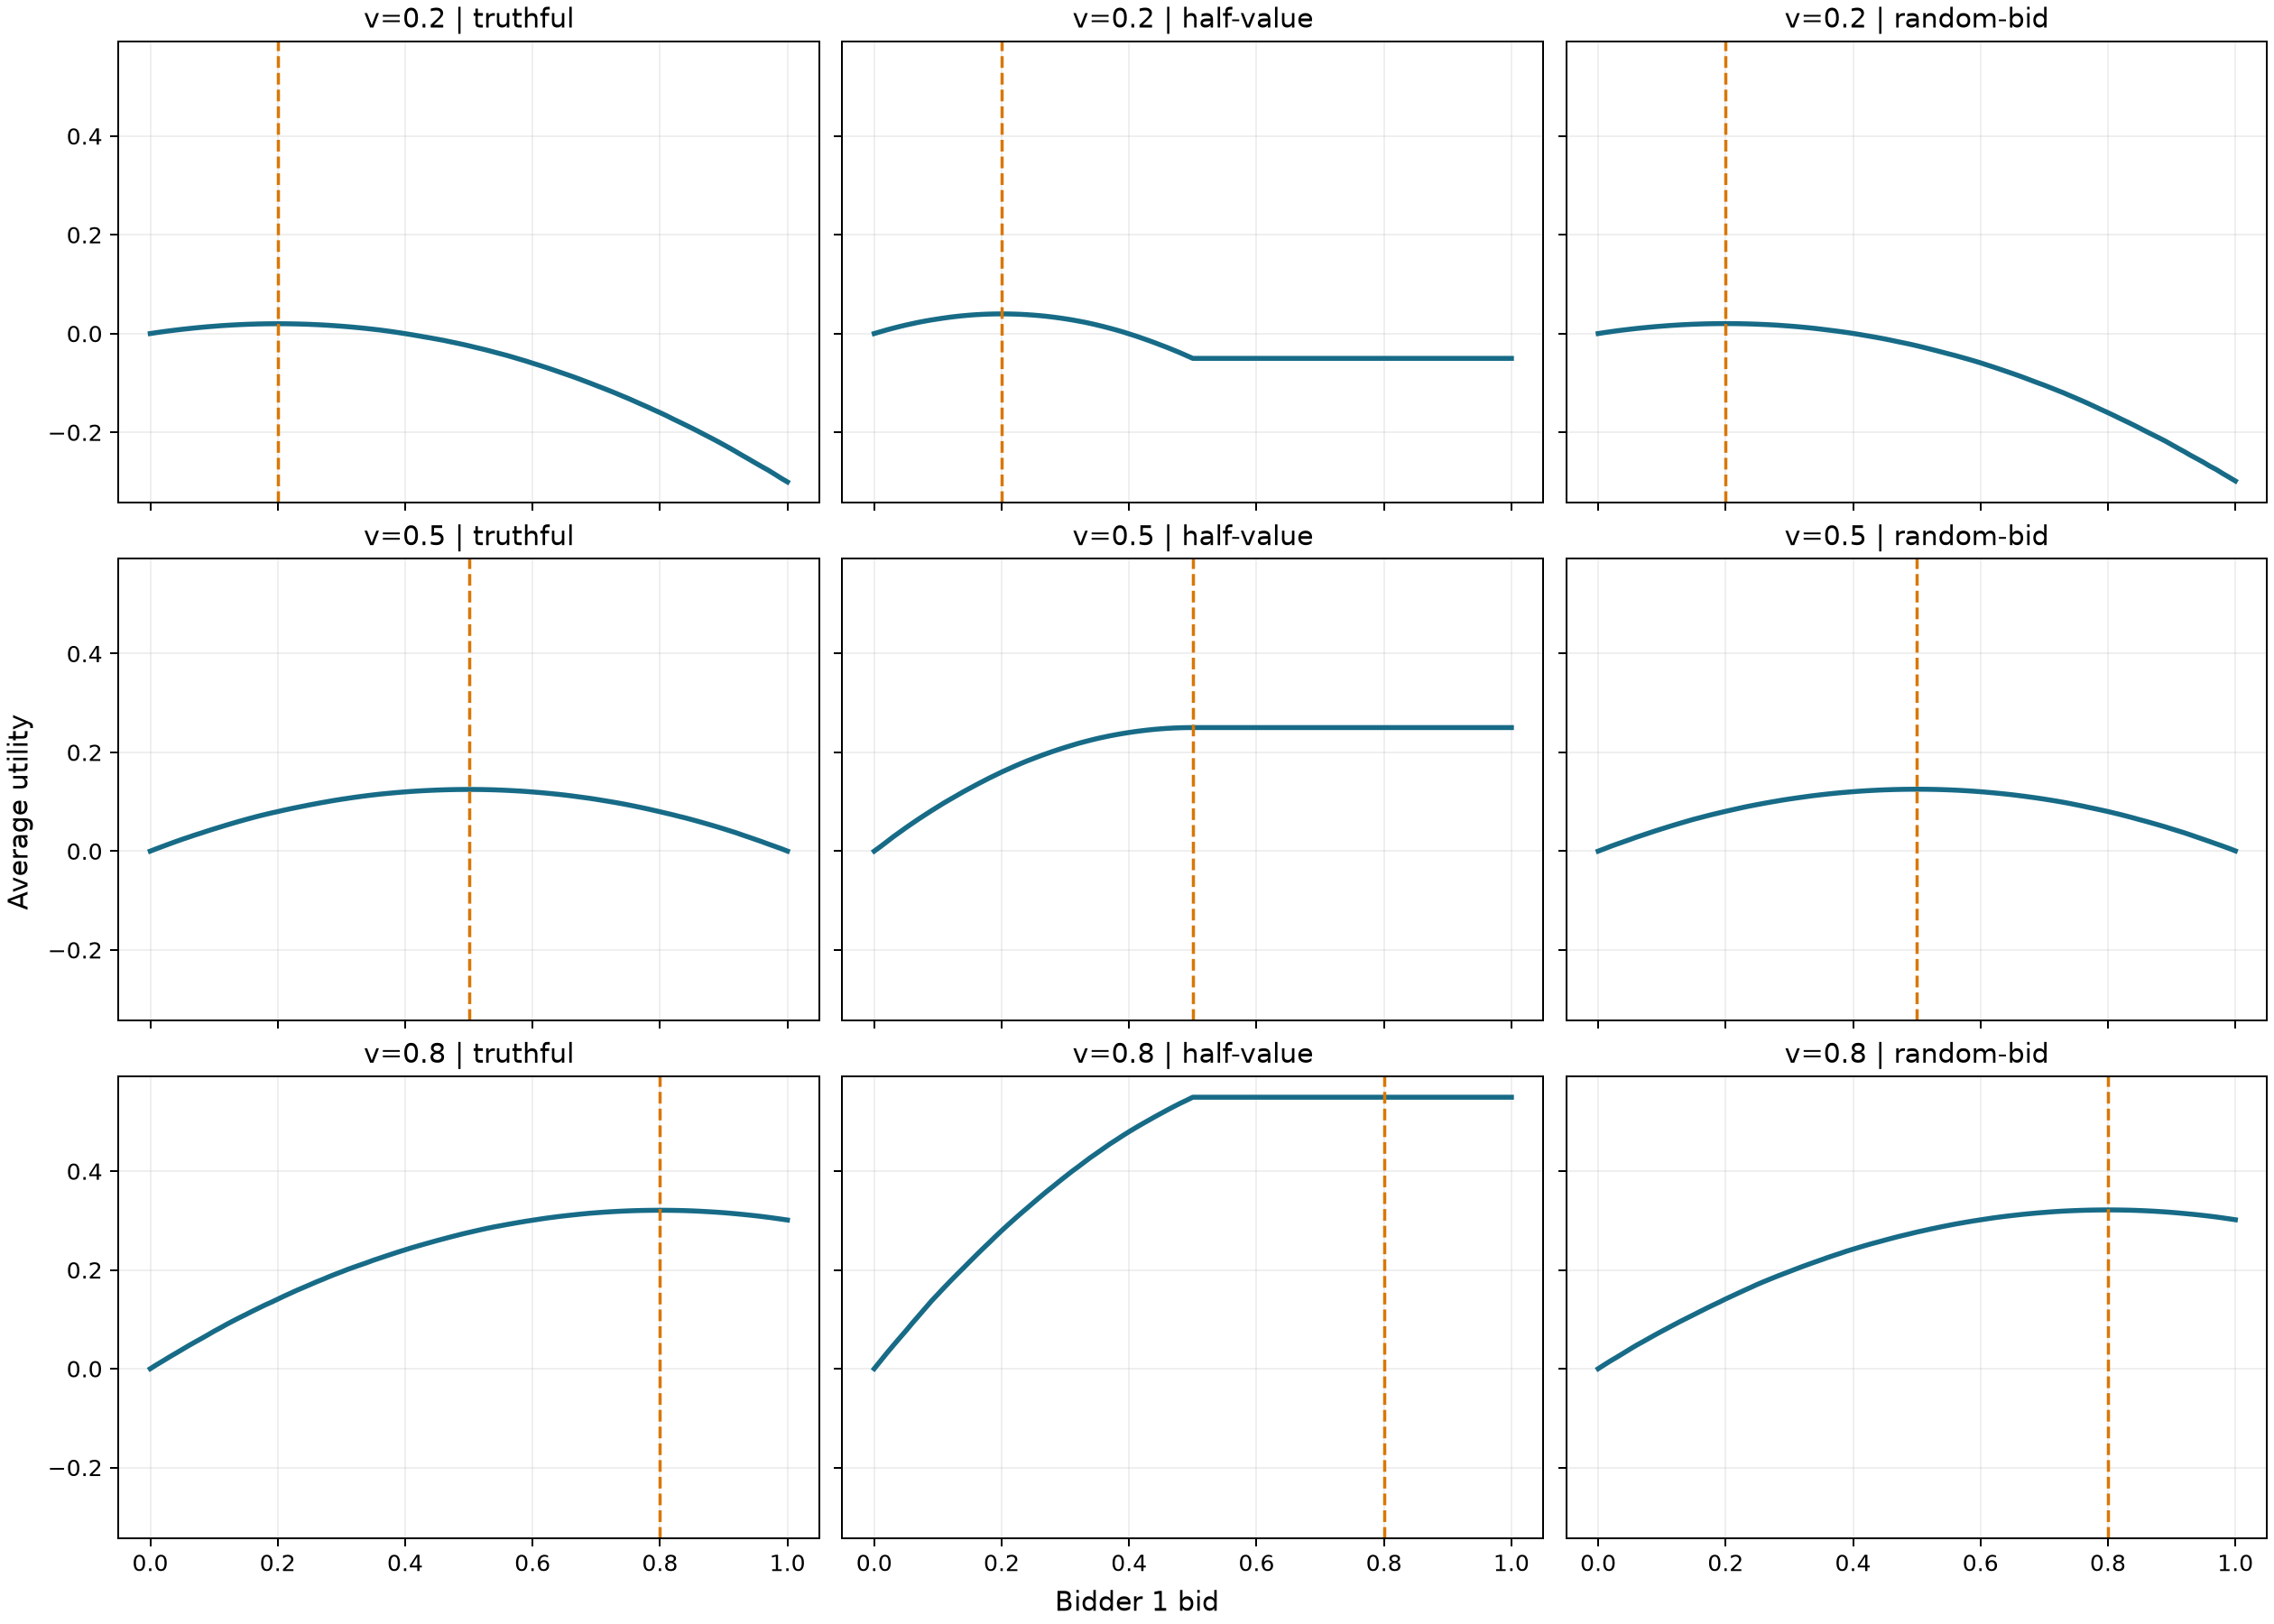
\includegraphics[width=0.98\linewidth]{figures/part1a_all_nine.png}
  \caption{Part 1A: bidder 1's average utility over the 101 tested bids, shown for all three values and rival strategies. The dashed line marks $b=v$.}
  \label{fig:part1a}
\end{figure}

\subsection{Fixed rival bid}

For a fixed rival bid $r$, any bid below $r$ loses and gives utility zero. A bid above $r$ wins and gives $v-r$. At $b=r$, the tie is split equally. If $r<v$, winning is profitable; if $r>v$, winning has negative utility. Bidding $b=v$ therefore gives the highest utility in each case. It may tie other bids in utility, so this is weak dominance rather than a unique optimum.

The nine combinations of $v\in\{0.2,0.5,0.8\}$ and $r\in\{0.1,0.4,0.9\}$ all passed the grid check: truthful bidding attained the maximum in 9 of 9 cases. Figure~\ref{fig:part1b} shows the corresponding best-response curves.

\begin{figure}[H]
  \centering
  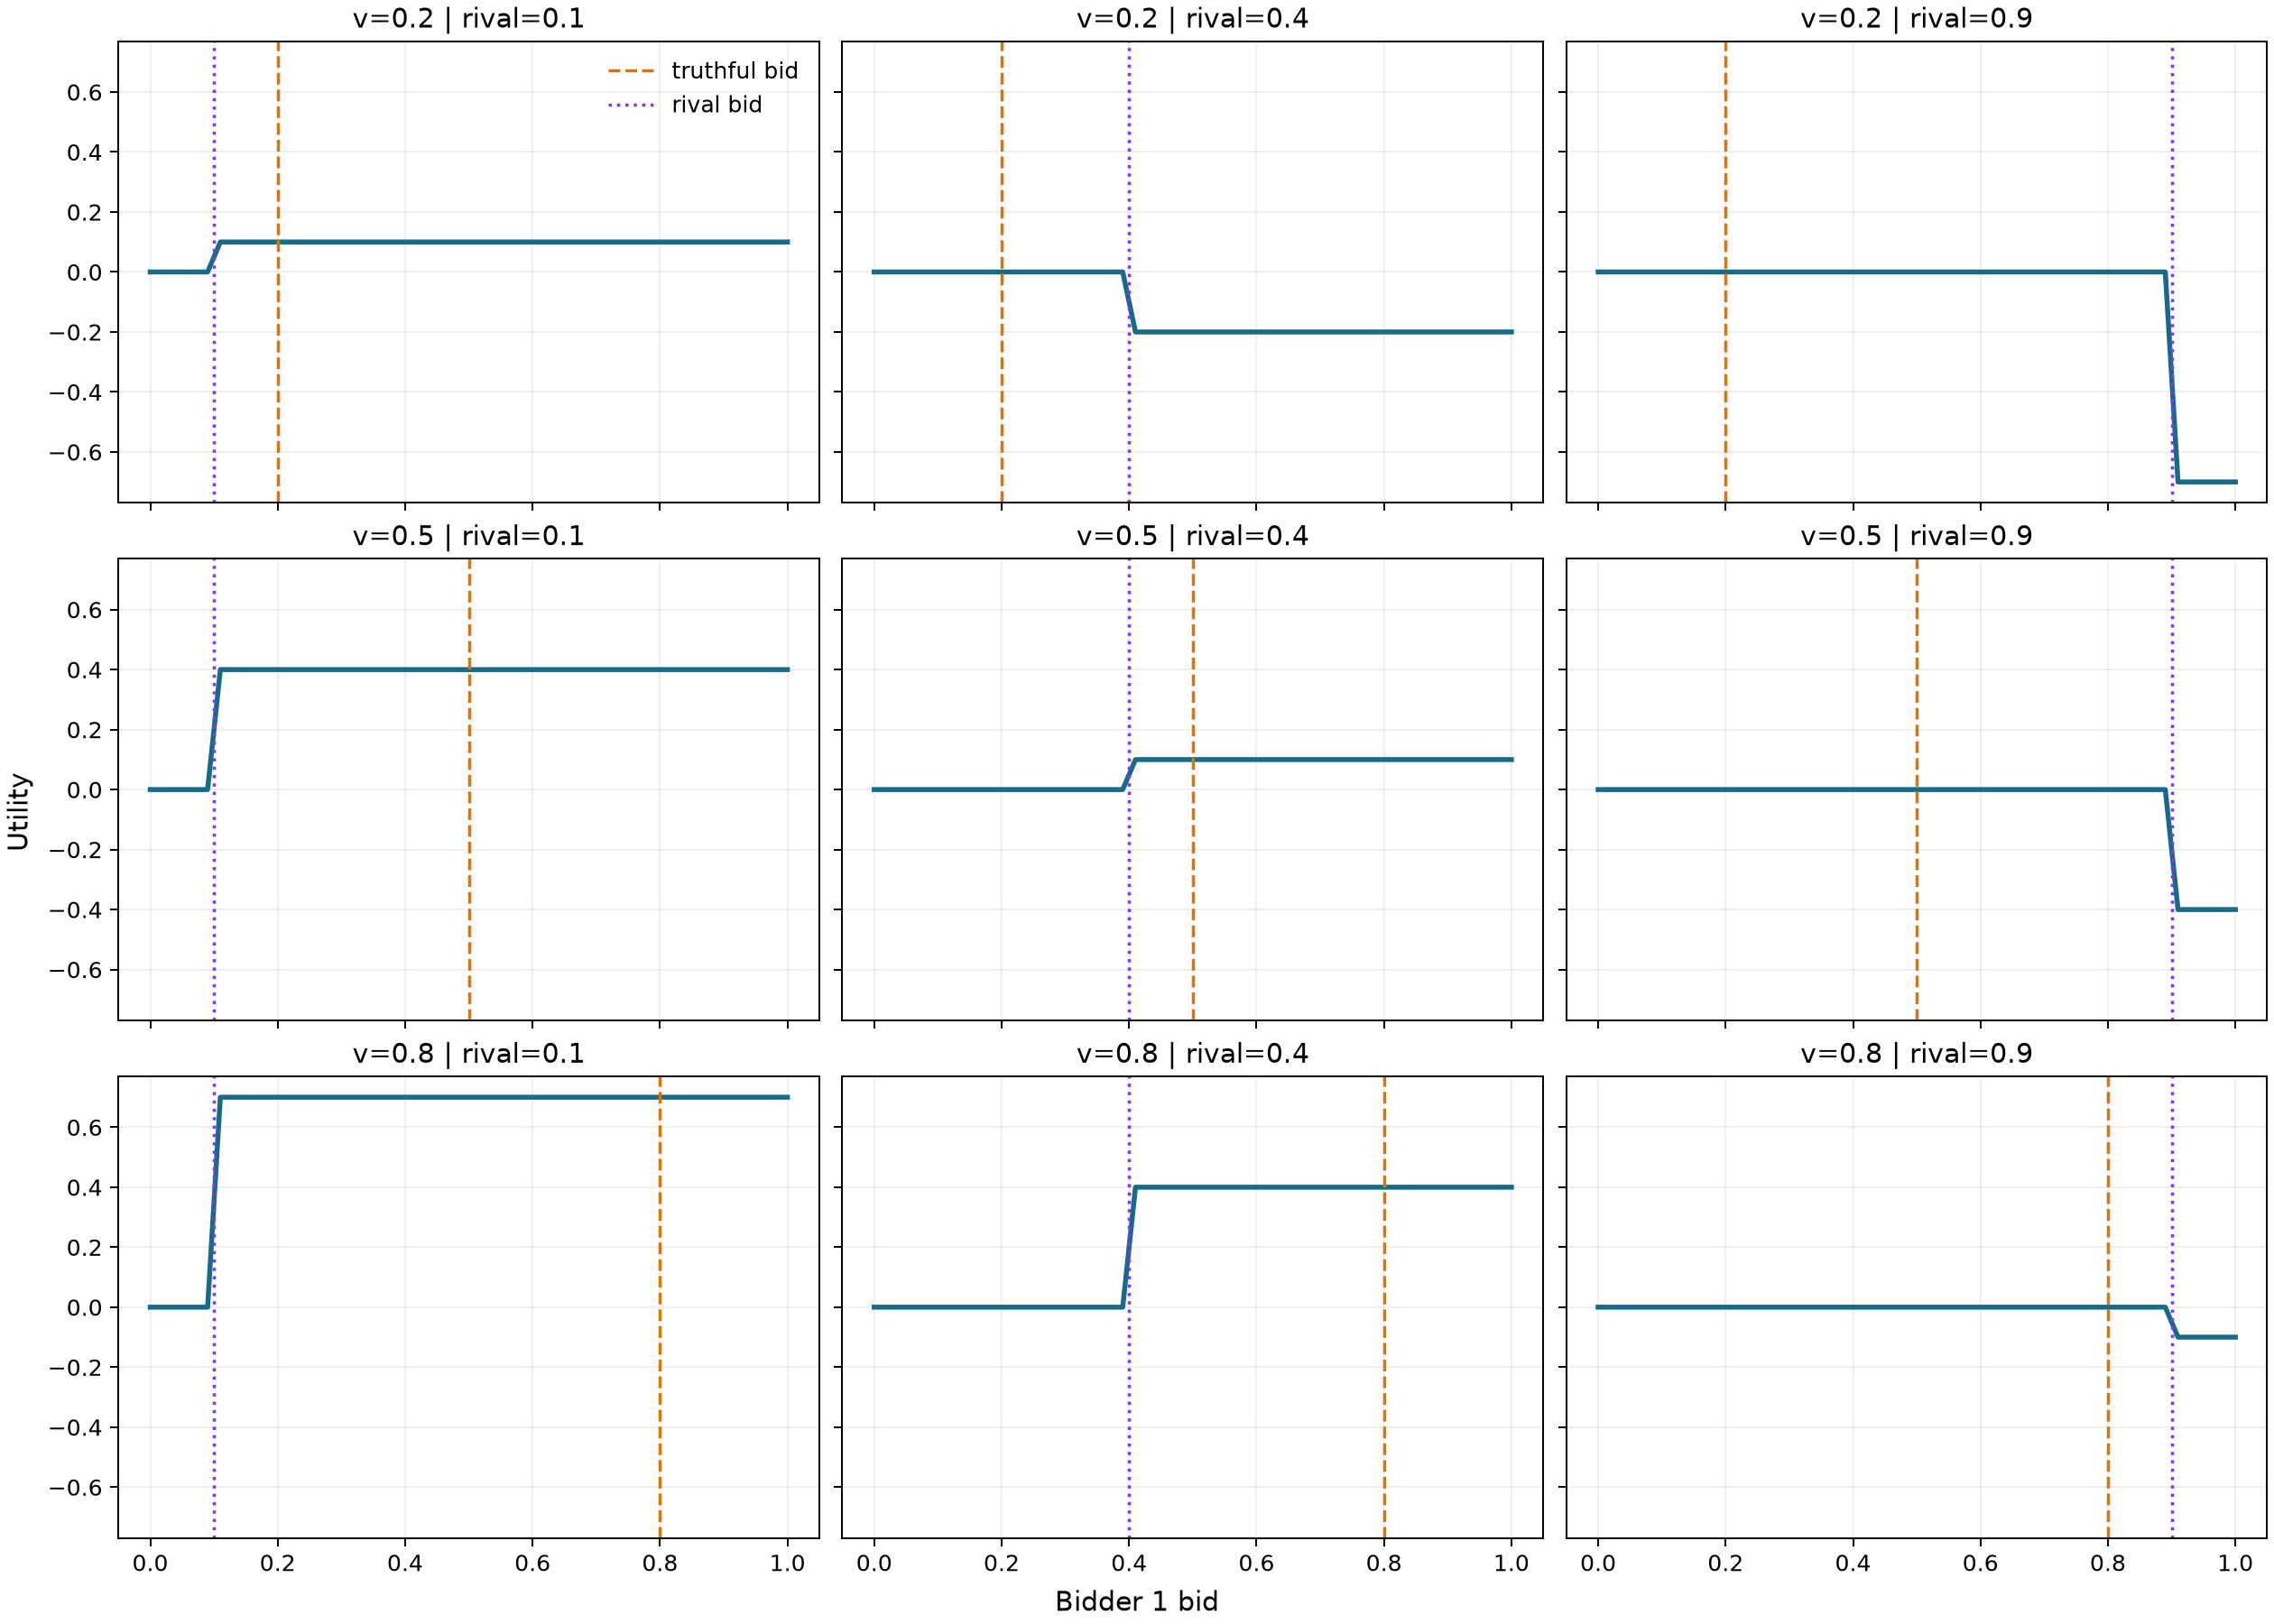
\includegraphics[width=0.98\linewidth]{figures/part1b_fixed_rival.png}
  \caption{Part 1B: utility against a fixed rival bid. The truthful bid and rival bid are marked in each panel.}
  \label{fig:part1b}
\end{figure}

\subsection{Two rivals}

With two rivals, $Y$ is the maximum of their bids. For truthful or independent random bids, $Y$ has density $2y$ on $[0,1]$, so
\[
  U_{\text{uniform},2}(b)=vb^2-\frac{2}{3}b^3.
\]
For two half-value rivals, the density of $Y$ is $8y$ on $[0,0.5]$. Hence
\[
  U_{\text{half},2}(b)=
  \begin{cases}
    4vb^2-\dfrac{8}{3}b^3, & 0\leq b\leq 0.5,\\
    v-\dfrac{1}{3}, & 0.5\leq b\leq 1.
  \end{cases}
\]
The observed truthful/random maxima remain at $b=v$. For half-value rivals, the empirical maximizing bid is $v=0.20$ for the lowest value and the interval $[0.50,1.00]$ at $v=0.50$ and $0.80$. The expected payoffs are lower than in the one-rival case because bidder 1 must outbid the maximum of two rival bids.

\begin{table}[H]
\centering
\caption{Maximum estimated utility in Part 1C's two-rival stochastic experiments.}
\label{tab:part1c}
\small
\begin{tabular}{ccccc}
\toprule
Value $v$ & Truthful rival strategy & Half-value strategy & Random-bid strategy & Maximizing bids\\
\midrule
0.20 & 0.002625 & 0.010687 & 0.002609 & $0.20$\\
0.50 & 0.041818 & 0.166607 & 0.041533 & $0.50$; half: $[0.50,1.00]$\\
0.80 & 0.170962 & 0.466525 & 0.170219 & $0.80$; half: $[0.50,1.00]$\\
\bottomrule
\end{tabular}
\end{table}

The fixed-rival extension sets both rival bids to $r$ and divides a tie among the three highest bidders. Truthful bidding attains the maximum in all 9 value/rival combinations. Figures~\ref{fig:part1c} and~\ref{fig:part1cfixed} show the stochastic and fixed-bid results, respectively.

\begin{figure}[H]
  \centering
  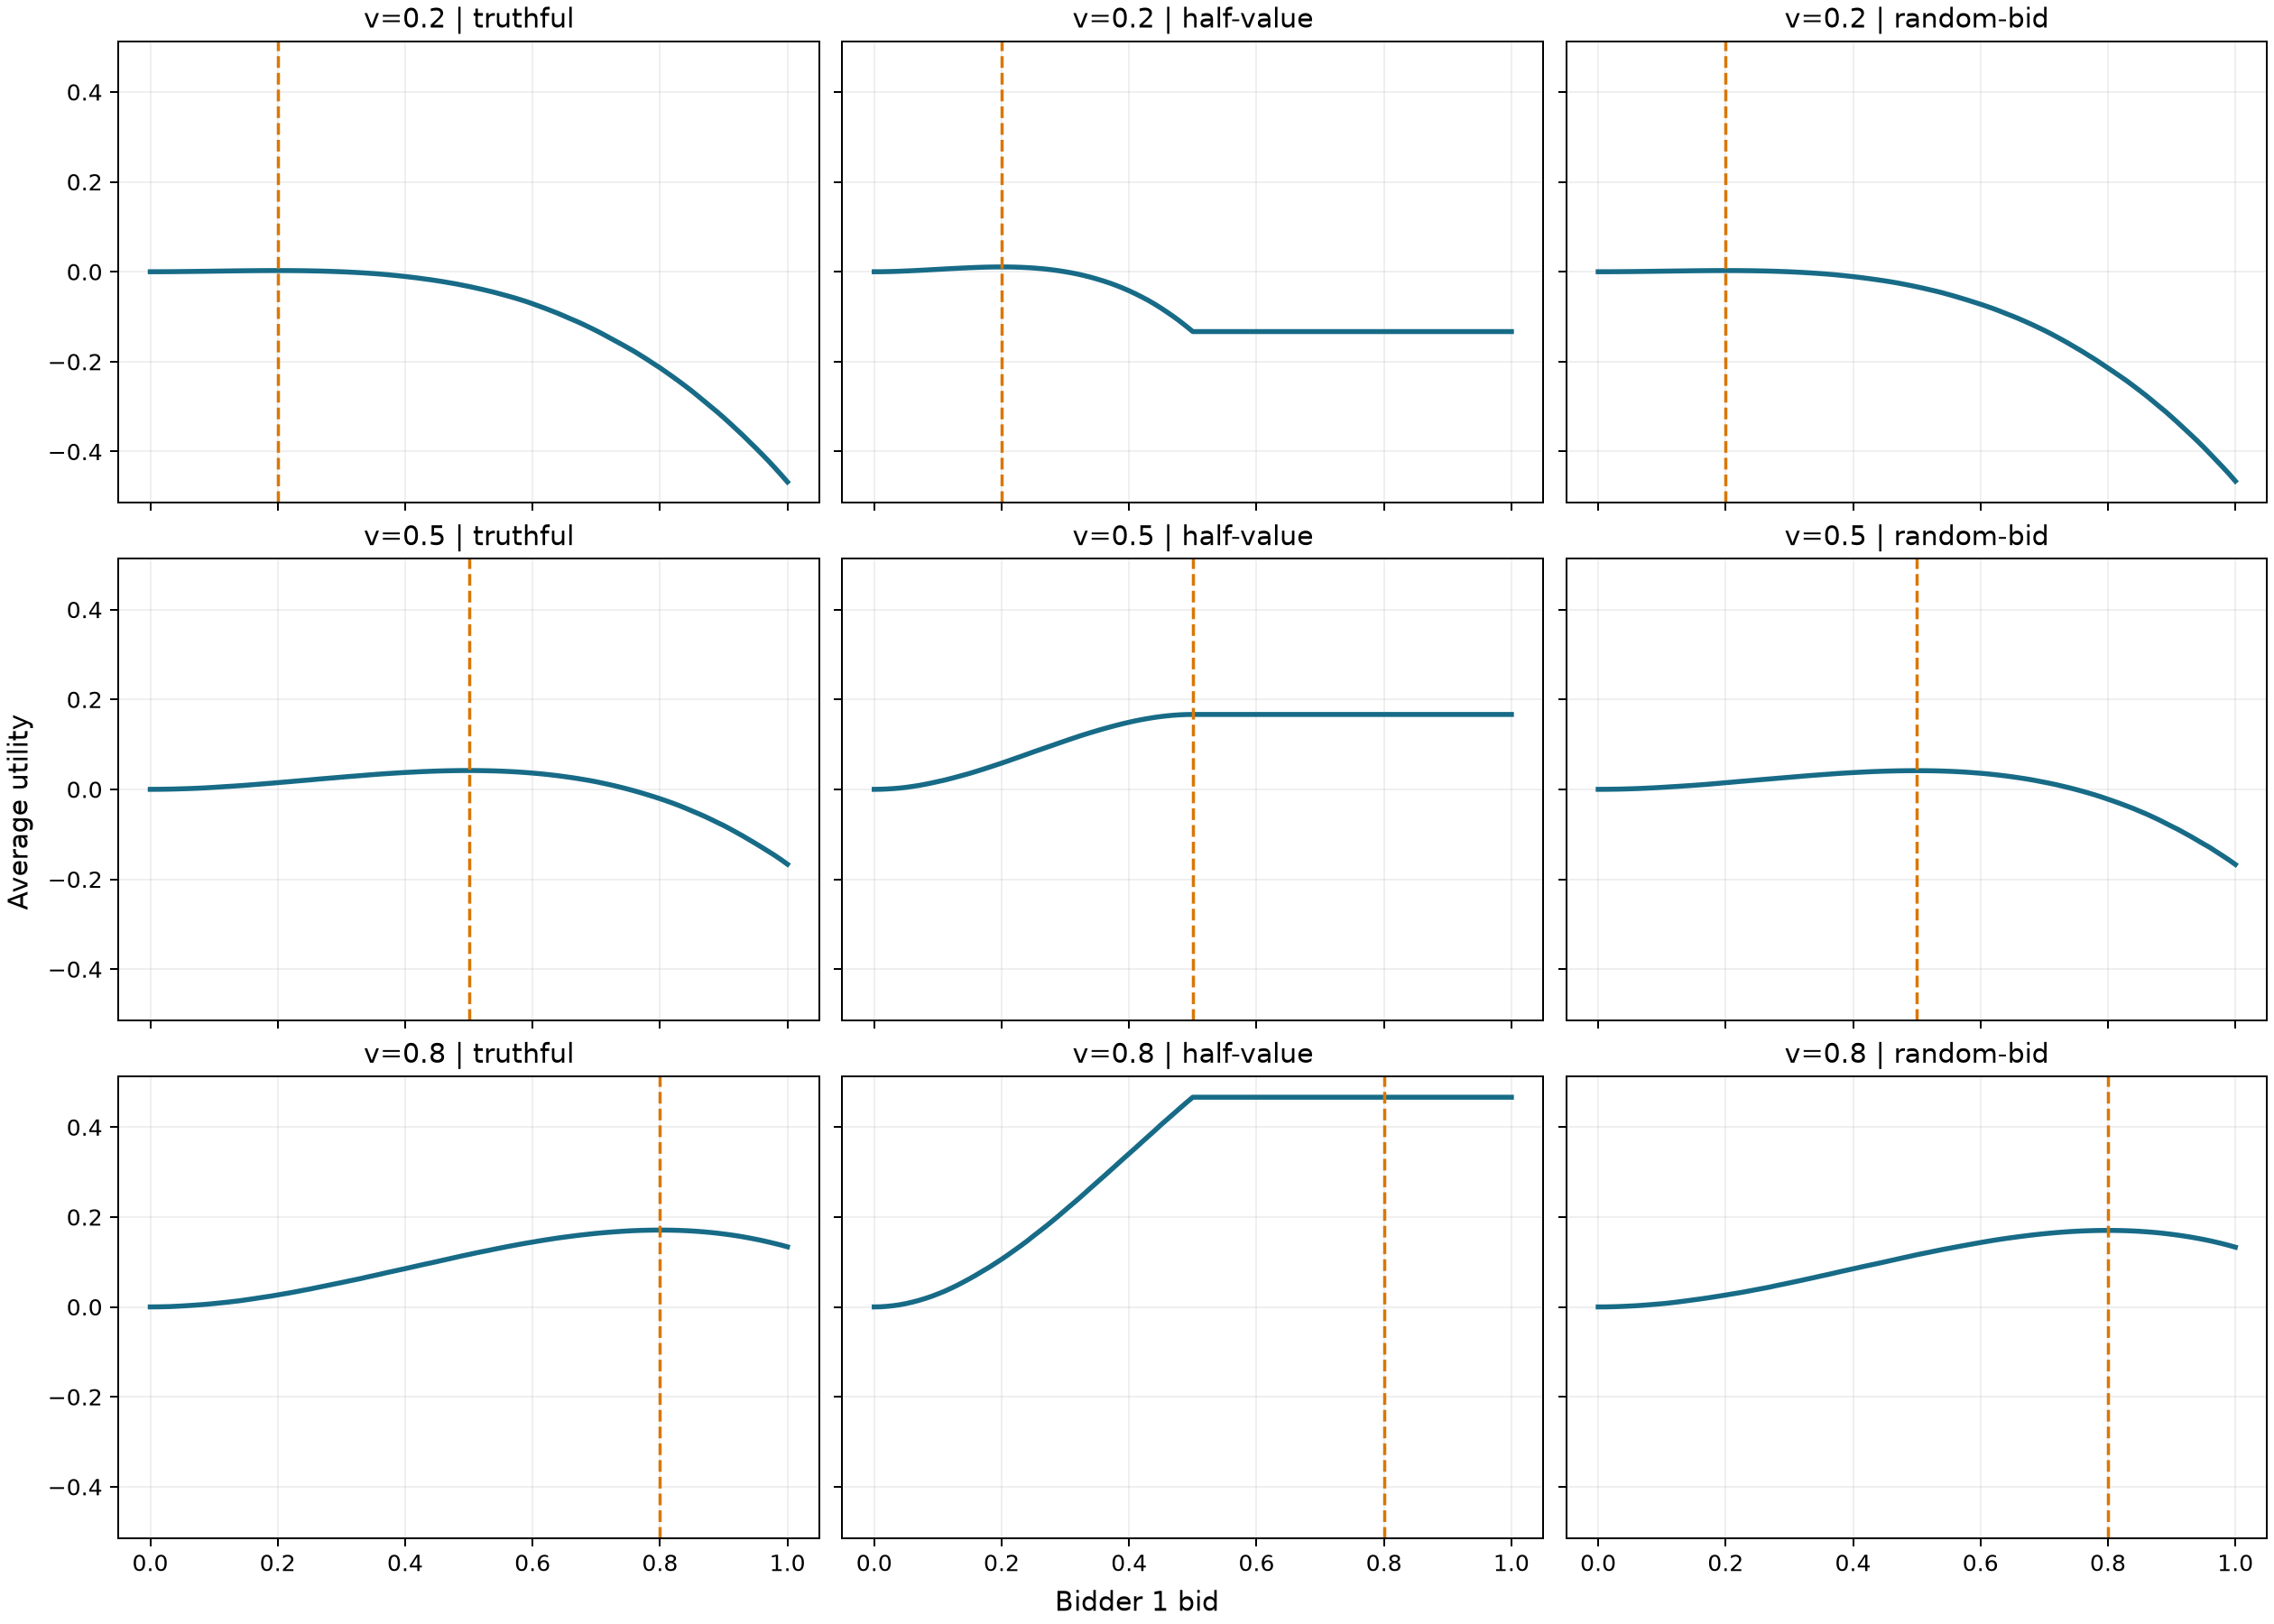
\includegraphics[width=0.98\linewidth]{figures/part1c_two_rivals.png}
  \caption{Part 1C: simulated utility curves with two rivals using the same strategy.}
  \label{fig:part1c}
\end{figure}

\begin{figure}[H]
  \centering
  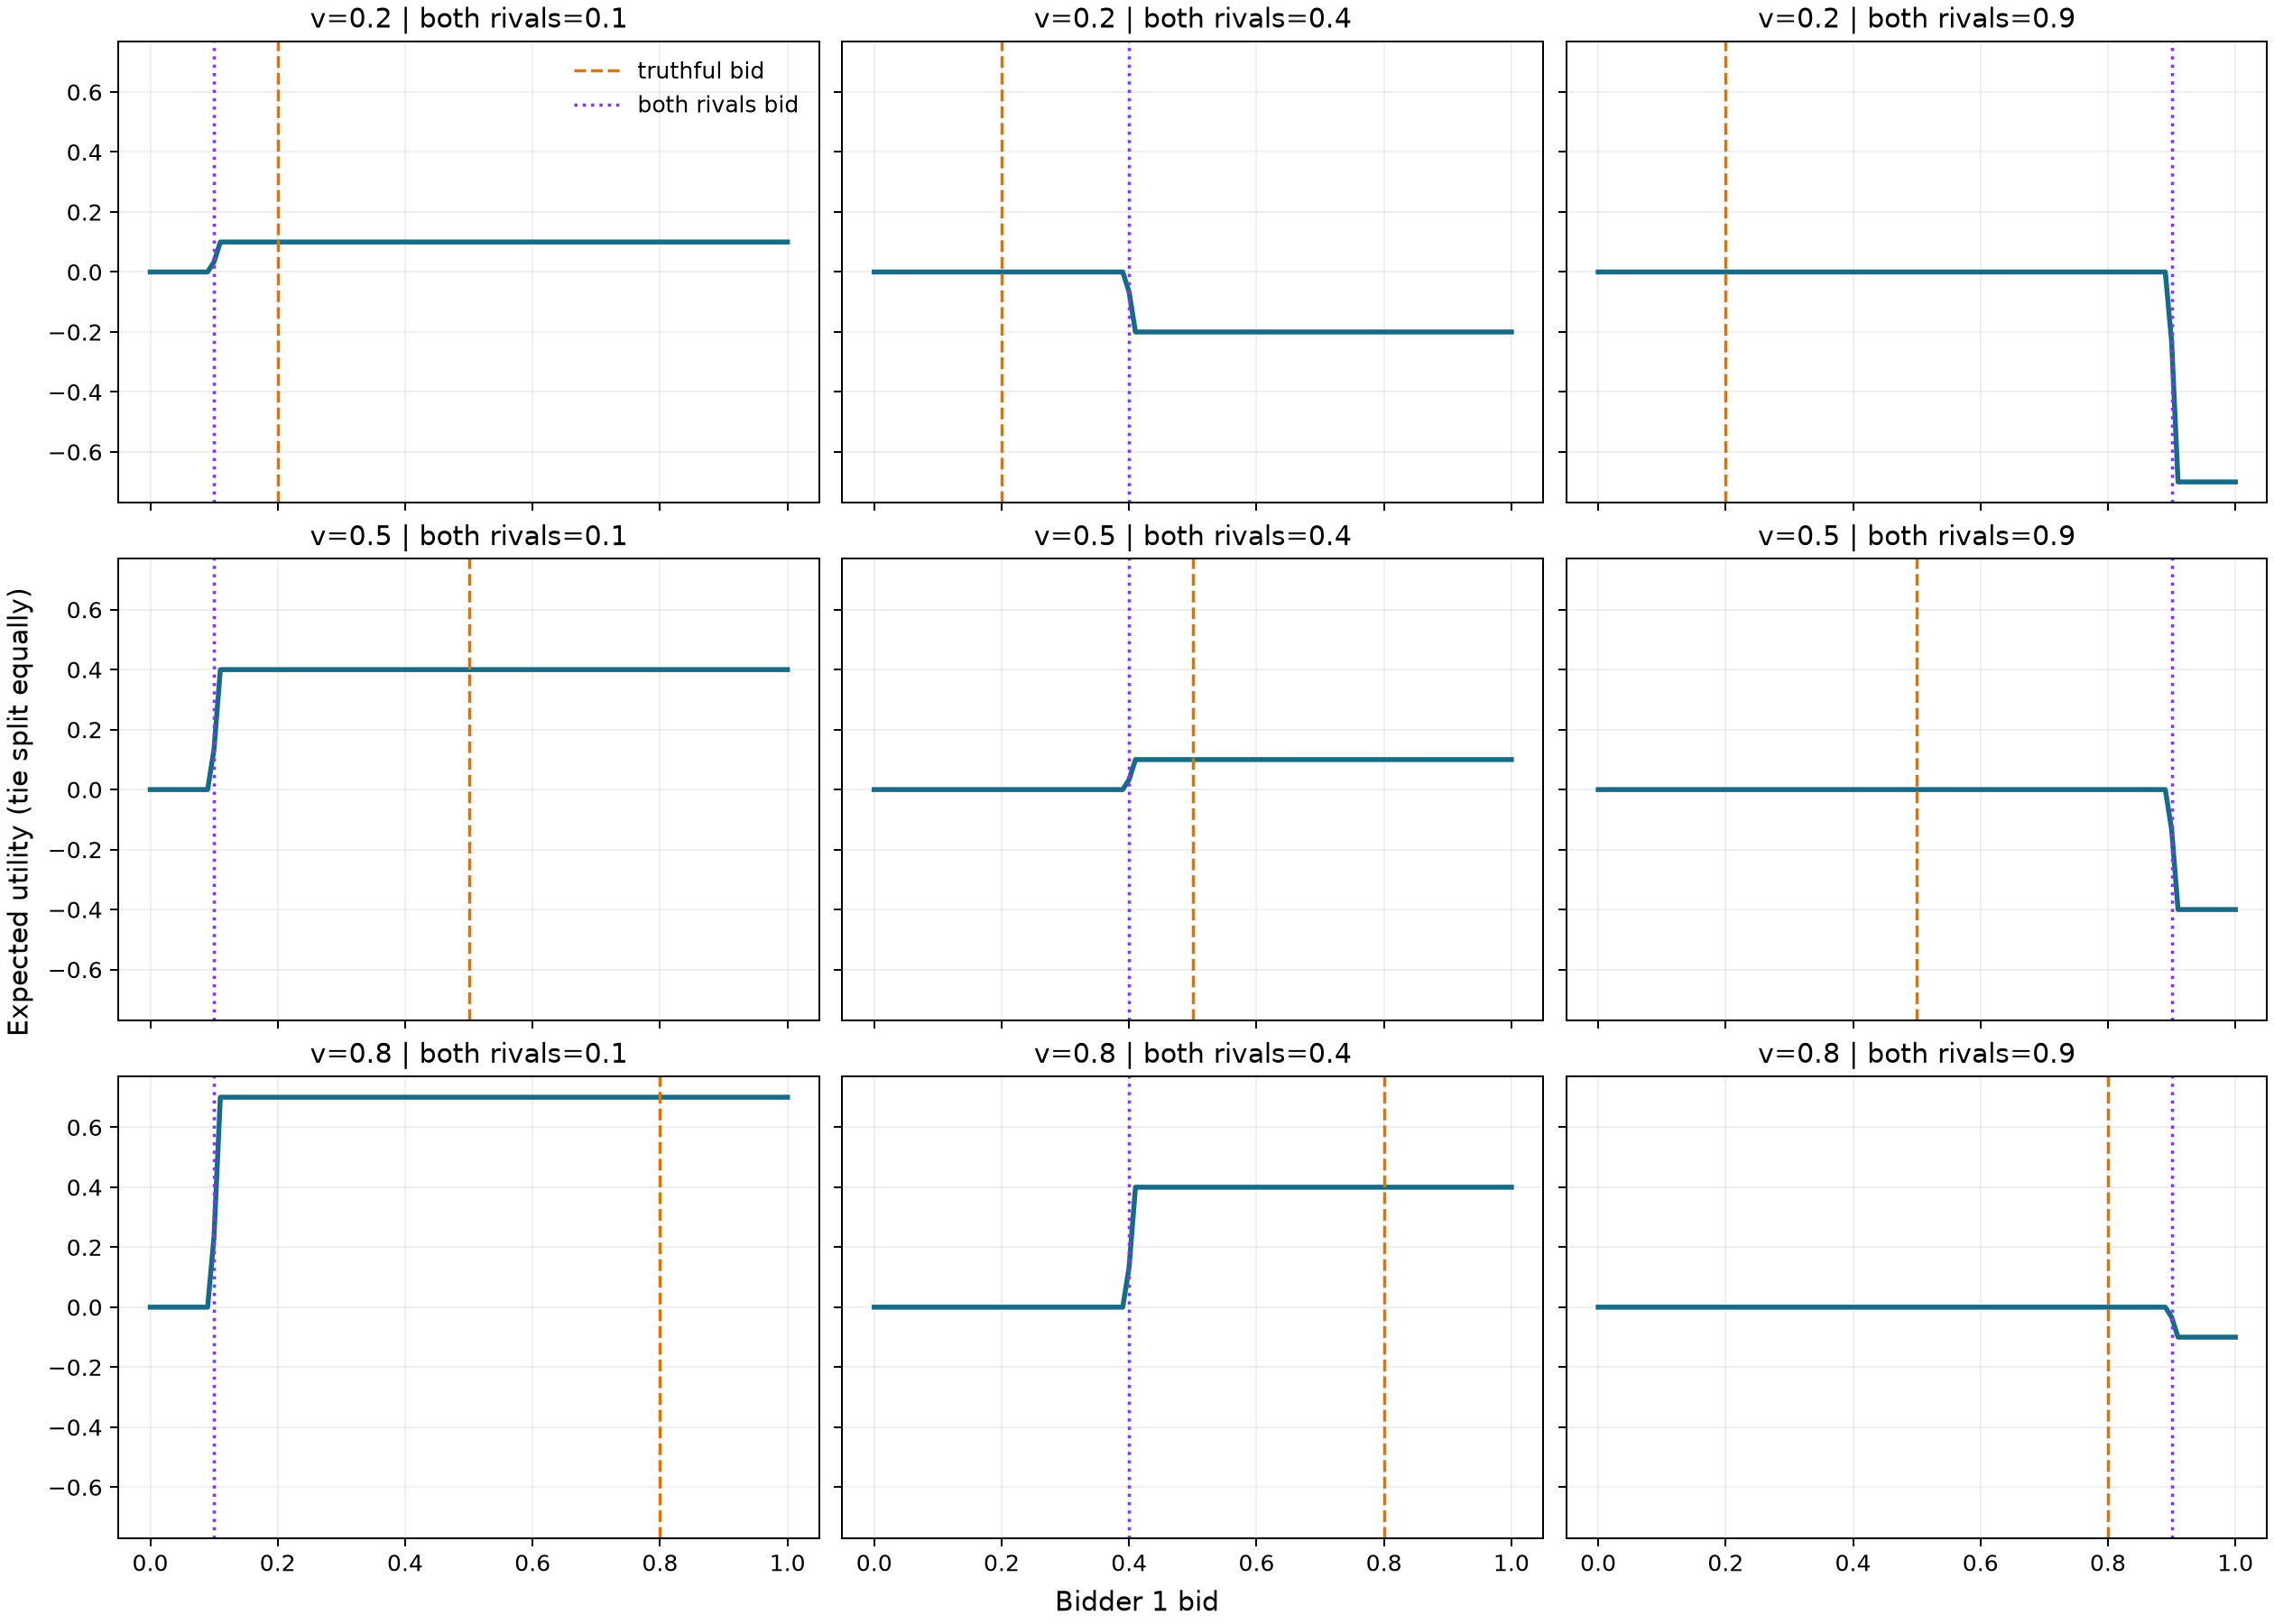
\includegraphics[width=0.98\linewidth]{figures/part1c_fixed_two_rivals.png}
  \caption{Part 1C fixed-bid check: both rivals bid the listed amount; ties at the shared bid are split three ways.}
  \label{fig:part1cfixed}
\end{figure}

\section{First-price auction}

For $n$ bidders, the $n-1$ rivals bid their equilibrium bid $\alpha x$, where $\alpha=(n-1)/n$ and $x$ is their uniform value. Bidder 1 has value $v=0.5$ and bids $b=kv$. For $b<\alpha$, each rival's bid is below $b$ with probability $b/\alpha$. Thus
\[
  \Pr(\text{win})=\min\left\{\left(\frac{kv}{\alpha}\right)^{n-1},1\right\},
  \qquad
  \mathbb{E}[u_1]=(v-kv)\Pr(\text{win}).
\]
The continuous optimum is $k=\alpha$. For the required discrete grid, the simulated maximum occurs at $k=0.5$ for $n=2$, and at $k=0.7$ for both $n=3$ and $n=4$. The continuous optimum for $n=4$ is $0.75$, between two grid points; on the grid, the exact expectation at $k=0.7$ is slightly above that at $k=0.8$.

At the continuous equilibrium multiplier, the conditional expected utility is $v^n/n$. For $v=0.5$, this gives $0.125000$, $0.041667$, and $0.015625$ for $n=2,3,4$, respectively. The exact expectations in Table~\ref{tab:part2} are evaluated at the discrete multipliers actually tested.

\begin{table}[H]
\centering
\caption{Part 2: best tested multiplier by empirical expected utility. Each $n$ uses 200,000 auctions.}
\label{tab:part2}
\small
\resizebox{\linewidth}{!}{%
\begin{tabular}{cccccccc}
\toprule
$n$ & Continuous $k^*$ & Best grid $k$ & Simulated $\mathbb{E}[u_1]$ & Exact at grid $k$ & Simulated win rate & Can lower fraction & Mean winner margin\\
\midrule
2 & 0.500 & 0.5 & 0.124734 & 0.125000 & 0.498935 & 1.000 & 0.124724\\
3 & 0.667 & 0.7 & 0.041496 & 0.041344 & 0.276640 & 1.000 & 0.135247\\
4 & 0.750 & 0.7 & 0.015145 & 0.015244 & 0.100965 & 1.000 & 0.146632\\
\bottomrule
\end{tabular}
}
\end{table}

The empirical expected utilities are close to their exact values at the selected grid multipliers. In every tested $n,k$ combination, the winner's bid was strictly above the runner-up, so the measured ``could pay less and still win'' fraction was $1.000$. This follows from continuous rival values and makes the binary fraction uninformative here; the mean winner margin adds context. Figure~\ref{fig:part2} plots payoff, win probability, the fraction with positive margin, and mean margin over the full multiplier grid.

\begin{figure}[H]
  \centering
  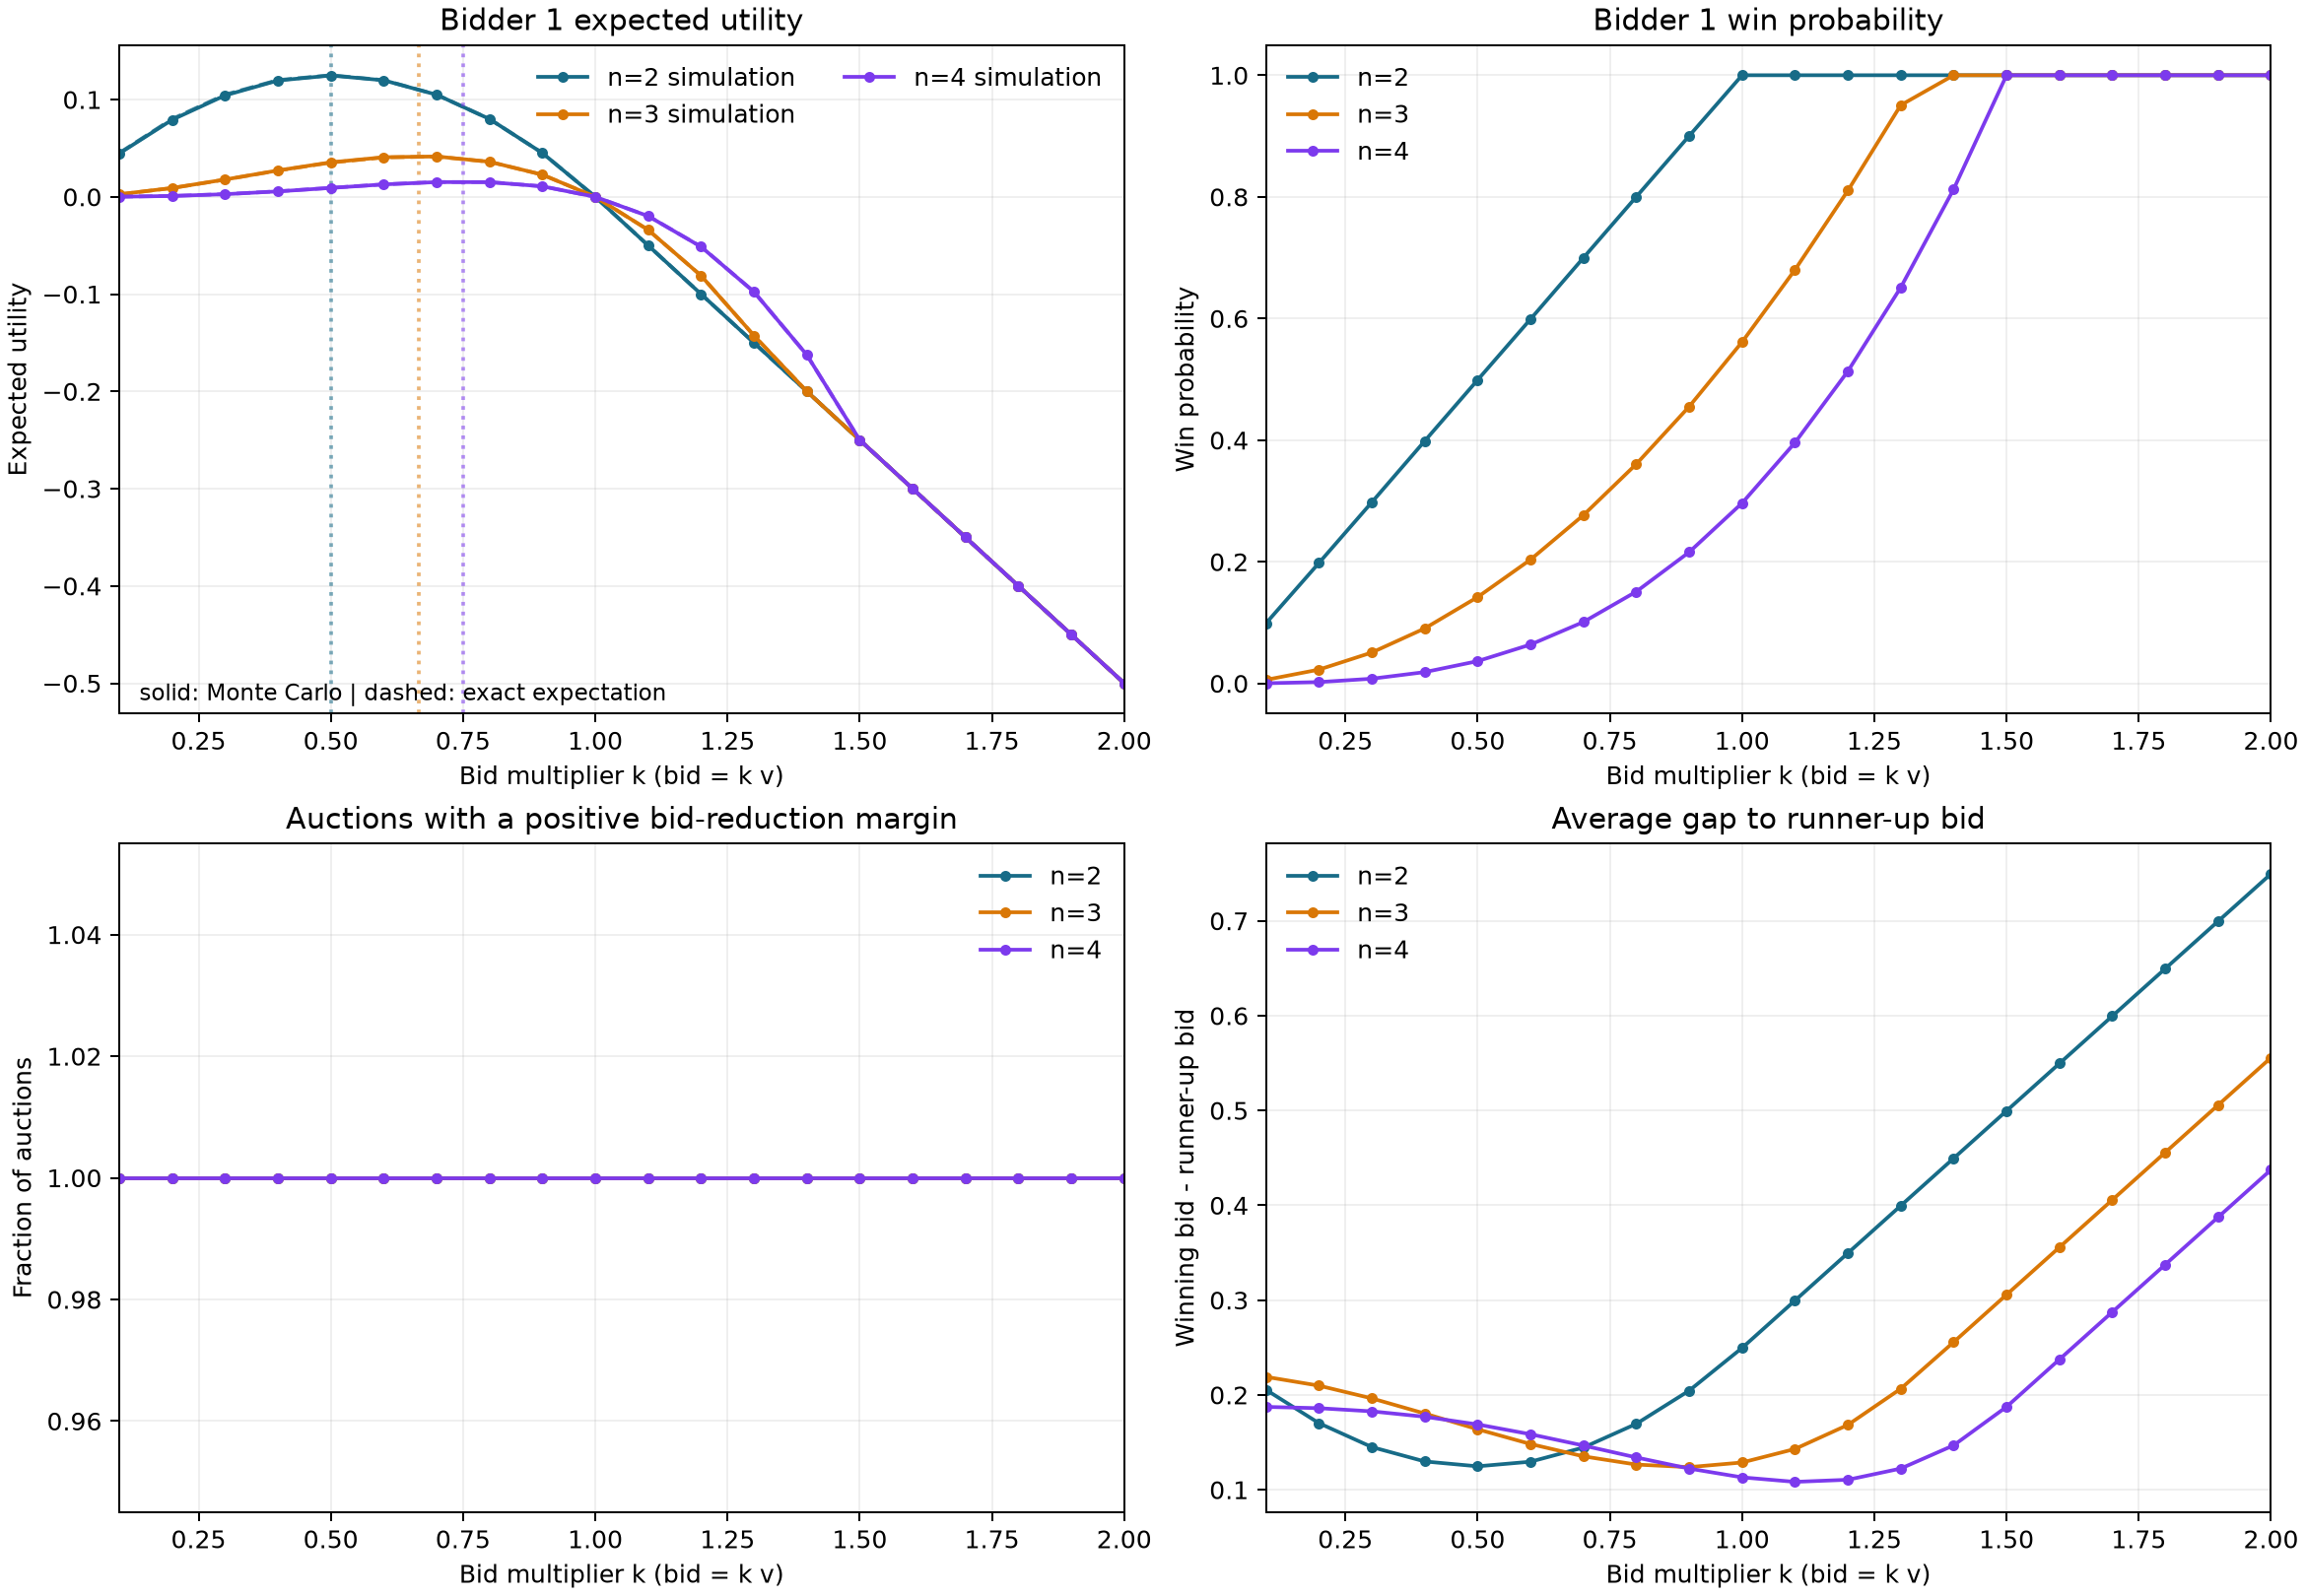
\includegraphics[width=0.98\linewidth]{figures/part2_first_price.png}
  \caption{Part 2: Monte Carlo payoff and win probability, plus the winner's reducible bid margin, for $n=2,3,4$. Dashed payoff curves are exact expectations.}
  \label{fig:part2}
\end{figure}

\section{VCG shortest-path procurement}

The network has eight directed edges, each controlled by a supplier with a private cost. The costs used are shown in Table~\ref{tab:edges}; they reproduce the transportation network referred to in the assignment and VCG discussion in \cite{shoham}.

\begin{table}[H]
\centering
\caption{Edge costs used in the VCG procurement network.}
\label{tab:edges}
\begin{tabular}{cccc}
\toprule
Edge & Cost & Edge & Cost\\
\midrule
AB & 3 & AC & 2\\
BD & 2 & BE & 1\\
CE & 3 & CF & 5\\
DF & 2 & EF & 1\\
\bottomrule
\end{tabular}
\end{table}

The candidate path costs are $c(ABEF)=5$, $c(ACEF)=6$, $c(ABDF)=7$, and $c(ACF)=7$. The efficient path is therefore ABEF. A selected supplier's VCG payment equals the cheapest path cost excluding its edge minus the cost of the other selected edges. The resulting outcome is:

\begin{table}[H]
\centering
\caption{Truthful VCG outcome. Payments are transfers to selected suppliers.}
\label{tab:vcg}
\begin{tabular}{ccccc}
\toprule
Edge & Selected & Payment & True cost & Supplier utility\\
\midrule
AB & Yes & 4 & 3 & 1\\
BE & Yes & 2 & 1 & 1\\
EF & Yes & 3 & 1 & 2\\
AC, BD, CE, CF, DF & No & 0 & -- & 0\\
\bottomrule
\end{tabular}
\end{table}

For example, excluding AB makes ACEF the cheapest remaining path at cost 6. The other selected edges BE and EF cost 2, so AB receives $6-2=4$. Similarly, BE is paid $6-(3+1)=2$, and EF is paid $7-(3+1)=3$. The mechanism pays 9 in total for a path whose true cost is 5.

The misreport sweep uses BE (on the selected path, true cost 1) and AC (off the selected path, true cost 2), with reports from 0 to 10 in increments of 0.5. BE's utility is 1 for reports through 2; above 2 it is excluded from the selected route and its utility becomes zero. AC's truthful utility is zero. Reports below 1 cause ACEF to be selected, but AC then receives payment 1, less than its true cost 2, so its utility is -1; reports from 1 upward give utility zero. Neither agent benefits from misreporting. The results illustrate the dominant-strategy truthfulness of the VCG pivot rule in this instance.

\begin{figure}[H]
  \centering
  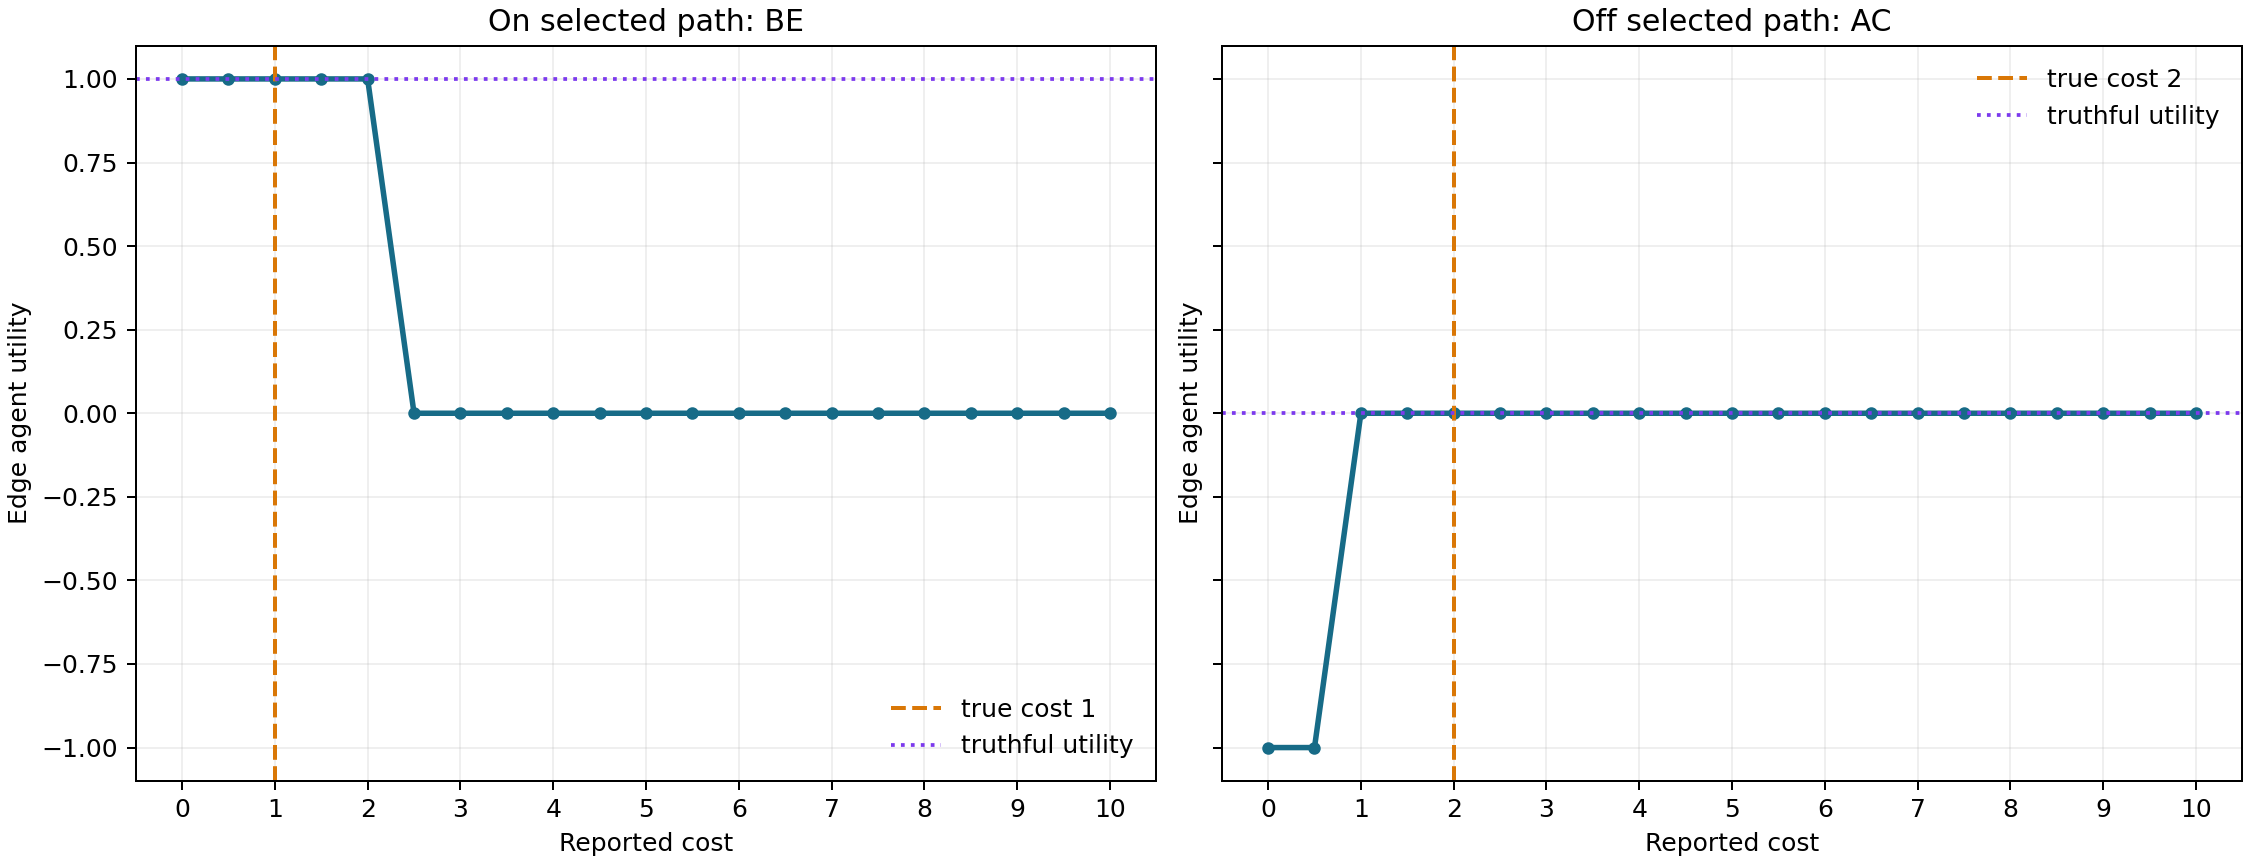
\includegraphics[width=0.98\linewidth]{figures/part3_vcg_misreports.png}
  \caption{Part 3: utility against reported cost for one selected edge (BE) and one unselected edge (AC).}
  \label{fig:part3}
\end{figure}

\section{Conclusion}

Across the tested second-price cases, truthful bidding attains the highest estimated utility, including with two rivals. The half-value rival creates flat regions of equally good bids when bidder 1's value is at least 0.5, but truthful bidding remains among them. In the first-price experiment, the empirical payoff peaks on the required grid at the multiplier closest to the symmetric equilibrium multiplier; the Monte Carlo utilities track their analytical values. Finally, the VCG mechanism selects ABEF and reproduces the requested transfers. The two misreport sweeps show no gain over truthful reporting.

\section*{Reproducibility}

Run the following commands from the project directory with the provided \texttt{as\_env} environment activated. They reproduce the plots and CSVs summarized above.

\begin{verbatim}
python part1a_second_price_single_rival.py --trials 100000 --seed 7
python part1b_second_price_fixed_rival.py
python part1c_second_price_two_rivals.py --trials 100000 --seed 19
python part2_first_price.py --trials 200000 --value 0.5 --seed 31
python part3_vcg_shortest_path.py
\end{verbatim}

The source is split into separate scripts for Parts 1A, 1B, 1C, 2, and 3. The combined interactive demonstration is provided separately as \texttt{demo/index.html}.

\begin{thebibliography}{9}
\bibitem{assignment4}
Assignment 4 handout, supplied course PDF.

\bibitem{shoham}
Y. Shoham and K. Leyton-Brown, \emph{Multiagent Systems: Algorithmic, Game-Theoretic, and Logical Foundations}, Cambridge University Press, 2009. Transportation-network VCG example; the assignment refers to Figure 7.3.
\end{thebibliography}

\end{document}
